\section[Concepts]{Quick review of $C^{++}$ concepts}
\subsection[Introduction]{History and goals}
\subsubsection{Origin of $C^{++}$}

\includeonlyframes{current}

\begin{frame}
  \frametitle{C/\cpp origins}
  \begin{minipage}{0.4\linewidth}
    \tikzstyle{old}=[ellipse,draw=black,fill=orange!30,thick,inner sep=2pt]
    \tikzstyle{new}=[rectangle,draw=black,fill=green!50,thick,inner sep=2pt]
    \tikzstyle{direct}=[<-,semithick]
    \tikzstyle{transverse}=[<-,dotted,semithick]
    \begin{tikzpicture}[->, node distance=.75cm, font=\tiny]
      \node[old] (Simula)      {Simula};
      \node[left of=Simula,node distance=1.5cm] {1967};
      \node[old] (BCPL) [right of=Simula, node distance=2cm] {BCPL};
      \node[old] (B) [below of=BCPL] {B}
      edge[transverse] (BCPL);
      \node[old] (KandRC) [below of=B] {K and R C}
      edge[transverse] (B);
      \node[left of=KandRC,node distance=3.5cm] {1978};
      \node[old] (ClassicC) [below of=KandRC] {Classic C}
      edge[direct] (KandRC);
      \node[old] (CwithClasses) [below of=Simula,node distance=3cm] {C with Classes}
      edge[transverse] (Simula)
      edge[transverse] (BCPL)
      edge[direct] (ClassicC);
      \node[left of=CwithClasses,node distance=1.5cm] {1980};
      \node[old] (EarlyC++) [below of=CwithClasses] {Early \cpp}
      edge[direct] (CwithClasses);
      \node[left of=EarlyC++,node distance=1.5cm] {1985};
      \node[old] (C89) [below of=ClassicC,node distance=2.25cm] {C89}
      edge[direct] (ClassicC)
      edge[transverse] (CwithClasses);
      \node[old] (ARMC++) [below of=EarlyC++] {ARM \cpp}
      edge[direct] (EarlyC++)
      edge[transverse] (C89);
      \node[left of=ARMC++,node distance=1.5cm] {1989};
      \node[old] (C++98) [below of=ARMC++] {\cpp98}
      edge[direct] (ARMC++)
      edge[transverse] (C89);
      \node[old] (C99) [below of=C89] {C99}
      edge[direct] (C89)
      edge[transverse] (ARMC++);
      \node[left of=C++98,node distance=1.5cm] {1998};
      \node[new] (C++11) [below of=C++98] {\cpp11}
      edge[direct] (C++98)
      edge[transverse] (C99);
      \node[left of=C++11,node distance=1.5cm] {2011};
      \node[new] (C11) [below of=C99] {C11}
      edge[direct] (C99)
      edge[transverse] (C++98);
      \node[new] (C++14) [below of=C++11] {\cpp14}
      edge[direct] (C++11);
      \node[left of=C++14,node distance=1.5cm] {2014};
    \end{tikzpicture}
  \end{minipage}
  \begin{minipage}{0.57\linewidth}
    \begin{tabular}{cc}
      \includegraphics[height=2.5cm]{ritchie.jpeg} & \includegraphics[height=2.5cm]{BjarneStroustrup.jpg} \\[-1ex]
      \tiny{C inventor} & \tiny{\cpp inventor} \\[-1ex]
      \scriptsize{Dennis M. Ritchie} & \scriptsize{Bjarne Stroustrup} \\
    \end{tabular}
    \begin{itemize}
      {\footnotesize
      \item Both C and \cpp are born in Bell Labs
      \item \cpp \it{almost} embeds C
      \item C and \cpp are still under development
      \item we will mainly discuss \cpp98
      }
    \end{itemize}
  \end{minipage}
\end{frame}

\subsubsection{Does it fit our needs ?}

\begin{frame}
  \frametitle{Why ic \cpp our language of choice ?}
  \pause
  \begin{block}{Adapted to large projects}
    \begin{itemize}
    \item strongly typed
    \item object oriented
    \item many available libraries
    \end{itemize}
  \end{block}
  \pause
  \begin{block}{Fast}
    \begin{itemize}
    \item as it's compiled (unlike Java or C\#)
    \item allows to go close to hardware
    \end{itemize}
  \end{block}
\end{frame}

\subsection[Basics]{Langage basics}

\begin{frame}[fragile]
  \frametitle{Hello World}
  \begin{cppcode}
    #include <iostream>

    // This is a function
    void print(int i) {
      std::cout << "Hello, world " << i << std::endl;
    }

    int main(int argc, char** argv) {
      int n = 3;
      for (int i = 0; i < n; i++) {
        print(i);
      }
      return 0;
    }
  \end{cppcode}
\end{frame}

\begin{frame}[fragile]
  \frametitle{Comments}
  \begin{cppcode}
    // simple comment for integer declaration
    int i;

    /* multiline comment
     * in case we need to say more
     */
    double d;

    /**
     * Best choice : doxygen compatible comments
     * \fn bool isOdd(int i)
     * \brief checks whether i is odd
     * \param i input
     * \return true if i is odd, otherwise false
     */
     bool isOdd(int i);
  \end{cppcode}
\end{frame}

\begin{frame}[fragile]
  \frametitle{Basic types(1)}
  \begin{cppcode}
    bool b = true;            // boolean, true or false
    
    char c = 'a';             // 8 bits ASCII char
    char* s = "a C string";   // array of chars ended by \0
    string t = "a C++ string";// class provided by the STL

    char c = -3;              // 8 bits signed integer
    unsigned char c = 4;      // 8 bits unsigned integer

    short int s = -444;       // 16 bits signed integer
    unsigned short s = 444;   // 16 bits unsigned integer
    short s = -444;           // int is optionnal
  \end{cppcode}
\end{frame}
\begin{frame}[fragile]
  \frametitle{Basic types(2)}
  \begin{cppcode}
    int i = -123456;          // 32 bits signed integer
    unsigned int i = 1234567; // 32 bits signed integer

    long l = 0L               // 32 or 64 bits (ptr size)
    unsigned long l = 0UL;    // 32 or 64 bits (ptr size)

    long long ll = 0LL;       // 64 bits signed integer
    unsigned long long l = 0ULL; // 64 bits unsigned integer

    float f = 1.23;           // 32 (23+7+1) bits float
    double d = 1.23E34;       // 64 (52+11+1) bits float
  \end{cppcode}
\end{frame}

\begin{frame}[fragile]
  \frametitle{Portable numeric types}
  \alert{One needs to include specific header}
  \begin{cppcode}
    #include <stdint.h>
    
    int8_t c = -3;     // 8 bits, replaces char
    uint8_t c = 4;     // 8 bits, replaces unsigned char

    int16_t s = -444;  // 16 bits, replaced short
    uint16_t s = 444;  // 16 bits, replaced unsigned short

    int32_t s = -0674; // 32 bits, replaced int
    uint32_t s = 0674; // 32 bits, replaced unsigned int

    int64_t s = -0x1bc;// 64 bits, replaced long long
    uint64_t s = 0x1bc;// 64 bits, replaced unsigned long long
    \end{cppcode}
\end{frame}

\begin{frame}[fragile]
  \frametitle{Static arrays}
  \begin{cppcode*}{linenos=false}
    int ai[4] = {1,2,3,4};
    int ai[] = {1,2,3,4};  // identical
    
    char ac[3] = {'a','b','c'};   // char array
    char ac[4] = "abc";           // valid C string
    char ac[4] = {'a','b','c',0}; // same valid string
    
    int i = ai[2];  // i = 3
    char c = ac[8]; // garbage
    int i = ai[4];  // also garbage !
  \end{cppcode*}
\end{frame}

\begin{frame}[fragile]
  \frametitle{Pointers}
  \begin{multicols}{2}
    \begin{cppcode*}{linenos=false,gobble=6}
      int i = 4;
      int *pi = &i;
      int j = *pi + 1;
      
      int ai[] = {1,2,3};
      int *pai = ai;
      int *paj = pai + 1;
      int k = *paj + 1;
      
      int *pak = k;
      int *pak = (int*)k;
      int l = *pak; // seg fault !
    \end{cppcode*}
    \onslide<2->{
      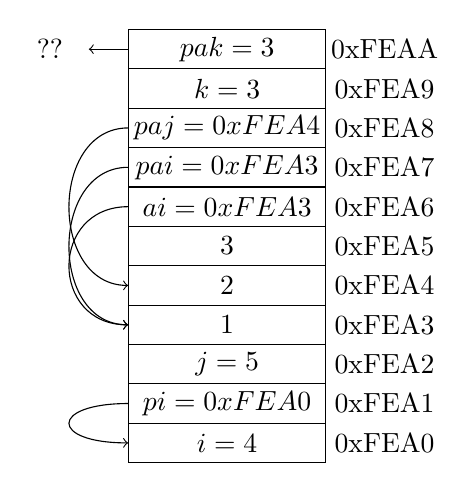
\begin{tikzpicture}
        \foreach \x/\xhex in {0,1,2,3,4,5,6,7,8,9,10/A}
        \draw node (stack\xhex) at (0,\x/2)
              [rectangle,minimum width=2.5cm,minimum height=0.5cm,draw] {}
              node at +(2,\x/2) {0xFEA\xhex};
        \onslide<3-> {\draw (0,0) node {$i = 4$};}
        \onslide<4-> {\draw (0,0.5) node {$pi = 0xFEA0$};}
        \onslide<5-> {\draw (0,1) node {$j = 5$};}
        \onslide<6-> {\draw (0,1.5) node {$1$};}
        \onslide<6-> {\draw (0,2) node {$2$};}
        \onslide<6-> {\draw (0,2.5) node {$3$};}
        \onslide<6-> {\draw (0,3) node {$ai = 0xFEA3$};}
        \onslide<7-> {\draw (0,3.5) node {$pai = 0xFEA3$};}
        \onslide<8-> {\draw (0,4) node {$paj = 0xFEA4$};}
        \onslide<9-> {\draw (0,4.5) node {$k = 3$};}
        \onslide<10-> {\draw (0,5) node {$pak = 3$};}
        \onslide<4-> {\draw[->] (stack1.west) .. controls +(left:1) and +(left:1) .. (stack0.west);}
        \onslide<6-> {\draw[->] (stack6.west) .. controls +(left:1) and +(left:1) .. (stack3.west);}
        \onslide<7-> {\draw[->] (stack7.west) .. controls +(left:1) and +(left:1) .. (stack3.west);}
        \onslide<8-> {\draw[->] (stack8.west) .. controls +(left:1) and +(left:1) .. (stack4.west);}
        \onslide<10-> {\draw[->] (stackA.west) -- +(left:.5);}
        \onslide<10-> {\draw node at +(-2.25,5) {??};}
      \end{tikzpicture}
    }
  \end{multicols}
\end{frame}

\begin{frame}[fragile]
  \frametitle{Dynamic Arrays}
  \begin{cppcode*}{linenos=false}
    #include <stdlib.h>
    #include <string.h>

    int *ai;     // pointer to random address
    int *ai = 0; // better. Can be tested

    // allocate array of 10 ints (not initialized)
    ai = (int*) malloc(10*sizeof(int));
    // and set them to 0
    memset(ai, 10, sizeof(int));

    // Both in one go
    ai = (int*) calloc(10, sizeof(int));
    
    // liberate memory
    free(ai);
  \end{cppcode*}
\end{frame}

\begin{frame}[fragile]
  \frametitle{Operators(1)}
  \begin{block}{Binary \& Assignment Operators}
    \begin{cppcode*}{linenos=false,gobble=4}
      int i = 1 + 4 - 2;  // 3
      i *= 3;             // 9
      i /= 2;             // 4
      i = 23 % i;         // modulo => 3
    \end{cppcode*}
  \end{block}
  \pause
  \begin{block}{Increment / Decrement \uncover<3->{\hfill \alert{\bf Use wisely}}}
    \begin{cppcode*}{linenos=false}
      int i = 0; i++; // i = 1
      int j = ++i;    // i = 2, j = 2
      int k = i++;    // i = 3, k = 2
      int l = --i;    // i = 2, l = 2
      int m = i--;    // i = 1, m = 2
    \end{cppcode*}
  \end{block}
\end{frame}

\begin{frame}[fragile]
  \frametitle{Operators(2)}
  \begin{block}{Bitwise and Assignment Operators}
    \begin{cppcode*}{linenos=false,gobble=4}
      int i = 0xee & 0x55;  // 0x44
      i |= 0xee;            // 0xee
      i ^= 0x55;            // 0xbb
      int j = ~0xee;        // 0xffffff11
      int k = 0x1f << 3;    // 0x78
      int l = 0x1f >> 2;    // 0x7
    \end{cppcode*}
  \end{block}
  \pause
  \begin{block}{Boolean Operators}
    \begin{cppcode*}{linenos=false,gobble=4}
      bool a = true;
      bool b = false;
      bool c = a && b;    // false
      bool d = a || b;    // true
      bool e = !d;        // false
    \end{cppcode*}
  \end{block}
\end{frame}

\begin{frame}[fragile]
  \frametitle{Operators(3)}
  \begin{block}{Comparison Operators}
    \begin{cppcode*}{linenos=false,gobble=4}
      bool a = (3 == 3);  // true
      bool b = (3 != 3);  // false
      bool c = (4 < 4);   // false
      bool d = (4 <= 4);  // true
      bool e = (4 > 4);   // false
      bool f = (4 >= 4);  // true
    \end{cppcode*}
  \end{block}
  \pause
  \begin{block}{Precedences \uncover<3->{\hfill \alert{\bf Don't use}\uncover<4->{\color{green} \bf\ - use parenthesis}}}
    \begin{cppcode*}{linenos=false}
      c &= 1+(++b)|(a--)*4%5^7; // ???
    \end{cppcode*}
  \end{block}
\end{frame}

\begin{frame}[fragile]
  \frametitle{struct}
  \begin{mdframed}[style=simplebox]
    \center ``members'' grouped together under one name
  \end{mdframed}
  \begin{multicols}{2}
    \begin{cppcode*}{linenos=false,gobble=6}
      struct Individual {
        unsigned char age;
        float weight;
        int userid;
      };

      Individual student;
      student.age = 25;
      student.weight = 78.5;
      student.userid = 1234;
    \end{cppcode*}
    \pause
    \columnbreak
    \begin{cppcode*}{linenos=false,gobble=6}
      Individual teacher = {
        .age = 45,
        .weight=67,
        .userid=5678 };
    \end{cppcode*}
    \onslide<2->{
      \begin{tikzpicture}
        \memorystack[nb blocks=10]
        \onslide<3-> {
          \memorypush{25,?,?,?}
          \memorypush{7,8,.,5}
          \memorypush{1,2,3,4}
          \memorystruct{1}{3}{student}
        }
        \onslide<4-> {
          \memorypush{45,?,?,?}
          \memorypush{6,7,.,0}
          \memorypush{5,6,7,8}
          \memorystruct{4}{6}{teacher}
        }
      \end{tikzpicture}
    }
  \end{multicols}
\end{frame}

\begin{frame}[fragile,label=current]
  \frametitle{union}
  \begin{mdframed}[style=simplebox]
    \center ``members'' packed together at same memory location
  \end{mdframed}
  \begin{multicols}{2}
    \begin{cppcode*}{linenos=false,gobble=6}
      union Duration {
        unsigned int seconds;
        unsigned short hours;
        unsigned char days;
      };

      Duration d1, d2, d3;
      d1.seconds = 259200;
      d2.hours = 72;
      d3.days = 3;
      d1.days = 3; // overwrite
    \end{cppcode*}
    \pause
    \columnbreak
    \onslide<2->{
      \vspace{2cm}
      \begin{tikzpicture}
        \memorystack
        \memorypush{25,?,?,?}
        \memorypush{7,8,.,5}
        \memorypush{1,2,3,4}
        \memorystruct{1}{3}{student}
        \memorypush{45,?,?,?}
        \memorypush{6,7,.,0}
        \memorypush{5,6,7,8}
        \memorystruct{4}{6}{teacher}
      \end{tikzpicture}
    }
  \end{multicols}
\end{frame}

\begin{frame}
  \frametitle{enum}
\end{frame}

\begin{frame}[fragile]
  \frametitle{Custom types}
  \begin{cppcode*}{linenos=false}
    typedef unsigned long long int ulli;
    ulli a = 12345;
  \end{cppcode*}
\end{frame}


\begin{frame}
  \frametitle{typedef}
\end{frame}

\begin{frame}
  \frametitle{Functions}
\end{frame}

\begin{frame}
  \frametitle{Preprocessor}
\end{frame}



\subsection[OO]{Object orientation}

\subsubsection{Classes}

\subsubsection{Inheritance}
\begin{frame}[fragile]
  \frametitle{Inheritance basics}
  \begin{cppcode}
  \end{cppcode}
\end{frame}

\begin{frame}[fragile]
  \frametitle{public / protected / private}
  \begin{minted}{c}
  \end{minted}
\end{frame}

\subsubsection{Operators}
\subsubsection{Exceptions}
